\documentclass[sigconf]{acmart}

\usepackage{tikz}
\usetikzlibrary{positioning, arrows.meta, shapes.geometric, shapes.multipart, fit, backgrounds}
\usepackage{listings}
\usepackage{xcolor}
\usepackage{booktabs}
\usepackage{amsmath}
\usepackage{float}
\usepackage{algorithm}
\usepackage{algorithmic}
\usepackage{pgfplots}
\pgfplotsset{compat=1.18}

\setcopyright{none}
\settopmatter{printacmref=false}
\pagestyle{plain}

\hypersetup{
  pdftitle={Prompt Contracts: A Formal Specification Language for Testing and Validating Large Language Model Outputs},
  pdfauthor={Philippos Melikidis},
  pdfsubject={Large Language Models, Prompt Engineering, Software Testing},
  pdfkeywords={Large Language Models, Prompt Engineering, Software Testing, Specification Languages, Contract-Based Design}
}

\lstdefinelanguage{json}{
  basicstyle=\ttfamily\footnotesize,
  numbers=left,
  numberstyle=\tiny,
  stepnumber=1,
  numbersep=5pt,
  showstringspaces=false,
  breaklines=true,
  frame=single,
  literate=
   *{0}{{{\color{blue}0}}}{1}
    {1}{{{\color{blue}1}}}{1}
    {2}{{{\color{blue}2}}}{1}
    {3}{{{\color{blue}3}}}{1}
    {4}{{{\color{blue}4}}}{1}
    {5}{{{\color{blue}5}}}{1}
    {6}{{{\color{blue}6}}}{1}
    {7}{{{\color{blue}7}}}{1}
    {8}{{{\color{blue}8}}}{1}
    {9}{{{\color{blue}9}}}{1}
    {:}{{{\color{red}{:}}}}{1}
    {,}{{{\color{red}{,}}}}{1}
    {\{}{{{\color{red}{\{}}}}{1}
    {\}}{{{\color{red}{\}}}}}{1}
    {[}{{{\color{red}{[}}}}{1}
    {]}{{{\color{red}{]}}}}{1},
}

\lstset{
  basicstyle=\ttfamily\scriptsize,
  breaklines=true,
  frame=single,
  numbers=left,
  numberstyle=\tiny,
  captionpos=b,
  showstringspaces=false,
  keywordstyle=\color{blue},
  commentstyle=\color{gray},
  stringstyle=\color{red},
  aboveskip=4pt,
  belowskip=4pt
}

\begin{filecontents*}{references.bib}
@article{meyer1992applying,
  title={Applying design by contract},
  author={Meyer, Bertrand},
  journal={Computer},
  volume={25},
  number={10},
  pages={40--51},
  year={1992},
  publisher={IEEE}
}

@misc{iso29119,
  title={{ISO/IEC/IEEE 29119-1:2013 Software and Systems Engineering -- Software Testing -- Concepts and Definitions}},
  author={{ISO/IEC/IEEE}},
  year={2013}
}

@book{russell2019human,
  title={Human Compatible: Artificial Intelligence and the Problem of Control},
  author={Russell, Stuart},
  year={2019},
  publisher={Viking},
  address={New York}
}

@misc{euaiact2024,
  author={{European Parliament and Council}},
  title={Regulation (EU) 2024/1689 on Artificial Intelligence (AI Act)},
  year={2024},
  howpublished={Official Journal of the European Union},
  note={Available at: \url{https://artificialintelligenceact.eu/}}
}

@article{hendrycks2021mmlu,
  title={Measuring Massive Multitask Language Understanding},
  author={Hendrycks, Dan and Burns, Collin and Basart, Steven and others},
  journal={arXiv preprint arXiv:2009.03300},
  year={2021}
}

@inproceedings{leike2018rewardmodeling,
  title={Scalable Agent Alignment via Reward Modeling},
  author={Leike, Jan and Krueger, David and Everett, Robert and others},
  booktitle={NeurIPS Workshops},
  year={2018}
}

@inproceedings{bender2021stochasticparrots,
  title={On the Dangers of Stochastic Parrots: Can Language Models Be Too Big?},
  author={Bender, Emily M and Gebru, Timnit and McMillan-Major, Angelina and Shmitchell, Shmargaret},
  booktitle={FAccT},
  year={2021}
}

@inproceedings{liang2022holistic,
  title={Holistic evaluation of language models},
  author={Liang, Percy and Bommasani, Rishi and Lee, Tony and Tsipras, Dimitris and Soylu, Dilara and Yasunaga, Michihiro and Zhang, Yian and Narayanan, Deepak and Wu, Yuhuai and Kumar, Ananya and others},
  booktitle={Proceedings of NeurIPS},
  year={2022}
}

@article{zheng2023judging,
  title={Judging LLM-as-a-judge with MT-bench and Chatbot Arena},
  author={Zheng, Lianmin and Chiang, Wei-Lin and Sheng, Ying and Zhuang, Siyuan and Wu, Zhanghao and Zhuang, Yonghao and Lin, Zi and Li, Zhuohan and Li, Dacheng and Xing, Eric and others},
  journal={Advances in NeurIPS},
  volume={36},
  year={2023}
}

@misc{langchain2023,
  author = {Chase, Harrison},
  title = {LangChain},
  year = {2023},
  howpublished = {\url{https://github.com/langchain-ai/langchain}}
}

@misc{trulens2023,
  author = {{TruEra}},
  title = {TruLens},
  year = {2023},
  howpublished = {\url{https://github.com/truera/trulens}}
}

@misc{ragas2023,
  author = {Shahul ES and Jithin James},
  title = {RAGAS},
  year = {2023},
  howpublished = {\url{https://github.com/explodinggradients/ragas}}
}

@misc{guidance2023,
  author = {{Microsoft Research}},
  title = {Guidance},
  year = {2023},
  howpublished = {\url{https://github.com/microsoft/guidance}}
}

@misc{openai2023structured,
  author = {{OpenAI}},
  title = {Structured Outputs in the API},
  year = {2023},
  howpublished = {\url{https://platform.openai.com/docs/guides/structured-outputs}}
}

@misc{ollama2023,
  author = {{Ollama}},
  title = {Ollama},
  year = {2023},
  howpublished = {\url{https://github.com/ollama/ollama}}
}

@inproceedings{openapi2017,
  title={The OpenAPI Specification},
  author={{OpenAPI Initiative}},
  year={2017},
  organization={Linux Foundation}
}

@article{ribeiro2020beyond,
  title={Beyond accuracy: Behavioral testing of NLP models with CheckList},
  author={Ribeiro, Marco Tulio and Wu, Tongshuang and Guestrin, Carlos and Singh, Sameer},
  journal={Proceedings of ACL},
  pages={4902--4912},
  year={2020}
}

@article{wang2023robustness,
  title={Robustness testing of language models: A survey},
  author={Wang, Xuezhi and Wei, Jason and Schuurmans, Dale and Le, Quoc and Chi, Ed and Zhou, Denny},
  journal={arXiv preprint arXiv:2303.12346},
  year={2023}
}

@article{ouyang2022training,
  title={Training language models to follow instructions with human feedback},
  author={Ouyang, Long and Wu, Jeffrey and Jiang, Xu and Almeida, Diogo and Wainwright, Carroll and Mishkin, Pamela and Zhang, Chong and Agarwal, Sandhini and Slama, Katarina and Ray, Alex and others},
  journal={Advances in NeurIPS},
  volume={35},
  pages={27730--27744},
  year={2022}
}

@article{wei2022chain,
  title={Chain-of-thought prompting elicits reasoning in large language models},
  author={Wei, Jason and Wang, Xuezhi and Schuurmans, Dale and Bosma, Maarten and Ichter, Brian and Xia, Fei and Chi, Ed and Le, Quoc and Zhou, Denny},
  journal={Advances in NeurIPS},
  volume={35},
  pages={24824--24837},
  year={2022}
}

@article{brown2020language,
  title={Language models are few-shot learners},
  author={Brown, Tom and Mann, Benjamin and Ryder, Nick and Subbiah, Melanie and Kaplan, Jared D and Dhariwal, Prafulla and Neelakantan, Arvind and Shyam, Pranav and Sastry, Girish and Askell, Amanda and others},
  journal={Advances in NeurIPS},
  volume={33},
  pages={1877--1901},
  year={2020}
}

@article{liu2023gpteval,
  title={G-Eval: NLG evaluation using GPT-4 with better human alignment},
  author={Liu, Yang and Iter, Dan and Xu, Yichong and Wang, Shuohang and Xu, Ruochen and Zhu, Chenguang},
  journal={Proceedings of EMNLP},
  year={2023}
}

@article{zhang2023safetybench,
  title={SafetyBench: Evaluating the safety of large language models},
  author={Zhang, Zhexin and Lei, Leqi and Wu, Lindong and Sun, Rui and Huang, Yongkang and Long, Chong and Liu, Xiao and Lei, Xuanyu and Tang, Jie and Huang, Minlie},
  journal={arXiv preprint arXiv:2309.07045},
  year={2023}
}

@article{zhao2023survey,
  title={A survey of large language models},
  author={Zhao, Wayne Xin and Zhou, Kun and Li, Junyi and Tang, Tianyi and Wang, Xiaolei and Hou, Yupeng and Min, Yingqian and Zhang, Beichen and Zhang, Junjie and Dong, Zican and others},
  journal={arXiv preprint arXiv:2303.18223},
  year={2023}
}

@article{achiam2023gpt,
  title={GPT-4 technical report},
  author={Achiam, Josh and Adler, Steven and Agarwal, Sandhini and Ahmad, Lama and Akkaya, Ilge and Aleman, Florencia Leoni and Almeida, Diogo and Altenschmidt, Janko and Altman, Sam and Anadkat, Shyamal and others},
  journal={arXiv preprint arXiv:2303.08774},
  year={2023}
}

@misc{reimers2019sentencebert,
  title={Sentence-BERT: Sentence Embeddings using Siamese BERT-Networks},
  author={Reimers, Nils and Gurevych, Iryna},
  journal={arXiv preprint arXiv:1908.10084},
  year={2019}
}

@book{efron1994bootstrap,
  title={An Introduction to the Bootstrap},
  author={Efron, Bradley and Tibshirani, Robert J},
  year={1994},
  publisher={Chapman and Hall/CRC}
}
\end{filecontents*}

\begin{document}

\title{Prompt Contracts: A Probabilistic Specification Language for Testing and Validating Large Language Model Outputs}

\author{Philippos Melikidis}
\affiliation{%
  \institution{Independent Researcher}
  \city{Bietigheim-Bissingen}
  \country{Germany}
}
\email{philipp.melikidis@gmail.com}

\begin{abstract}
Large Language Models (LLMs) function as stochastic, untyped interfaces lacking formal specifications. We introduce PCSL v0.3, the first probabilistic contract language for LLM prompt testing with statistical validation. Through N-sampling with configurable aggregation (majority/all/any) and bootstrap confidence intervals, PCSL quantifies reliability across 5 tasks (classification, extraction, summarization, RAG, tool-calls) totaling 1,247 fixtures. Evaluation demonstrates 100\% validation success with enforce mode (0\% repair), 92\% with assist (68\% repair vs. 12\% no-validation baseline). Bootstrap 95\% CIs confirm statistical significance. Semantic checks (similarity, LLM-as-judge) extend beyond structural validation. PCSL operationalizes compliance-as-code: artifact types map to ISO/IEC/IEEE 29119 test documentation, execution modes satisfy EU AI Act Articles 9-15. Implementation overhead: \(<\)5ms validation, 2.1\(\times\) latency for N=5 sampling. One-command reproduction via Docker (\texttt{make eval-full}) achieves deterministic results with seed=42.
\end{abstract}

\keywords{Large Language Models, Prompt Engineering, Software Testing, Probabilistic Contracts, Compliance}

\maketitle

\section{Introduction}

Large Language Models function as \textit{untyped, stochastic interfaces}: prompts map inputs to probabilistic outputs without formal behavioral guarantees~\cite{bender2021stochasticparrots}. Consider an LLM as \( f_\theta: \mathcal{X} \to P(\mathcal{Y}) \) where \( \theta \) are learned parameters and \( P(\mathcal{Y}) \) denotes a probability distribution over outputs. Unlike deterministic APIs with explicit contracts (e.g., \texttt{classify: String → \{A, B, C\}}), LLM outputs vary across runs, making traditional contract testing insufficient.

This gap becomes critical as LLMs deploy in regulated domains~\cite{euaiact2024}. The EU AI Act mandates transparency, auditability, and robustness testing for high-risk AI systems. Yet prompt engineering lacks the specification infrastructure available to traditional software: no type checking, no contract enforcement, no systematic validation with statistical confidence.

\textbf{Research Problem.} How can we define, validate, and enforce behavioral contracts for probabilistic LLM interfaces while ensuring reproducibility and regulatory compliance?

\textbf{Contributions.} This work presents:
\begin{enumerate}
\item \textbf{Probabilistic specification language}: PCSL v0.3 with N-sampling, aggregation policies (majority/all/any/first), and bootstrap confidence intervals for statistical validation (Section 3).
\item \textbf{Expanded evaluation}: Five tasks (1,247 fixtures) with structural and semantic checks, demonstrating 92\% validation success (assist) vs. 12\% baseline, with 95\% CI [0.89, 0.94] (Section 5).
\item \textbf{Compliance framework}: Formal mapping of PCSL artifacts to ISO 29119 test documentation and EU AI Act requirements, operationalizing compliance-as-code (Section 4.4).
\end{enumerate}

\section{Related Work}

\subsection{Contract-Based Testing}

Design-by-contract~\cite{meyer1992applying} formalizes software specifications through preconditions, postconditions, and invariants for deterministic functions. PCSL extends this to probabilistic functions by (1) N-sampling to estimate satisfaction probability, (2) aggregation policies to handle output variance, and (3) tolerance thresholds \(\tau\) for statistical validation.

OpenAPI~\cite{openapi2017} provides machine-readable REST API contracts. PCSL adopts this artifact-based design: Prompt Definitions (PD), Expectation Suites (ES), and Evaluation Profiles (EP) serve as versioned, provider-agnostic specifications.

\subsection{LLM Testing Frameworks}

CheckList~\cite{ribeiro2020beyond} introduces behavioral testing for NLP models through manually crafted test cases but lacks formal specification language and provider-agnostic execution. HELM~\cite{liang2022holistic} and MMLU~\cite{hendrycks2021mmlu} focus on model benchmarking, not individual prompt contract validation. LangChain~\cite{langchain2023} abstracts LLM development but provides limited systematic testing. Table~\ref{tab:comparison} summarizes key differences.

\begin{table}[t]
\centering
\caption{LLM Testing Frameworks Comparison}
\label{tab:comparison}
\scriptsize
\begin{tabular}{@{}lccccc@{}}
\toprule
\textbf{Framework} & \textbf{Contracts} & \textbf{Multi-Prov.} & \textbf{CI/CD} & \textbf{Semantic} & \textbf{Probabilistic} \\
\midrule
HELM~\cite{liang2022holistic} & \(\times\) & \checkmark & \(\times\) & \(\times\) & \(\times\) \\
LangChain~\cite{langchain2023} & \(\times\) & \checkmark & \(\times\) & \(\times\) & \(\times\) \\
Guidance~\cite{guidance2023} & \(\times\) & Limited & \(\times\) & \(\times\) & \(\times\) \\
OpenAI Struct.~\cite{openai2023structured} & Partial & \(\times\) & \(\times\) & \(\times\) & \(\times\) \\
CheckList~\cite{ribeiro2020beyond} & Manual & \checkmark & Partial & \(\times\) & \(\times\) \\
\textbf{PCSL v0.3 (ours)} & \checkmark & \checkmark & \checkmark & \checkmark & \checkmark \\
\bottomrule
\end{tabular}
\end{table}

\subsection{AI Safety and Regulation}

The EU AI Act~\cite{euaiact2024} mandates transparency (Article 13), record-keeping (Article 12), and accuracy validation (Article 15). ISO/IEC/IEEE 29119~\cite{iso29119} codifies software testing principles including traceability and reproducibility. PCSL uniquely bridges these requirements through formal artifact mapping (Section 4.4) and comprehensive audit trails.

\subsection{Research Gap}

Existing tools lack: (1) formal probabilistic specification language with statistical confidence bounds, (2) semantic validation beyond structural checks, (3) operational compliance mapping to ISO 29119 and EU AI Act. PCSL addresses all three.

\section{PCSL: Formal Specification}

\subsection{Core Definitions}

A \textit{prompt contract} \( \mathcal{C} = \langle \mathcal{P}, \mathcal{E}, \mathcal{X} \rangle \) consists of:
\begin{itemize}
\item \( \mathcal{P} \): Prompt Definition specifying template and I/O expectations
\item \( \mathcal{E} = \{e_1, \ldots, e_m\} \): Expectation Suite of validation checks
\item \( \mathcal{X} \): Evaluation Profile with fixtures, targets, and execution config
\end{itemize}

Each check \( e_i: \Omega \to \{\text{pass}, \text{fail}\} \) evaluates output \( o \in \Omega \). Contract satisfaction for a single output:
\[
\text{sat}(\mathcal{C}, o) \iff \bigwedge_{i=1}^{m} e_i(o) = \text{pass}
\]

\subsection{Probabilistic Semantics}

Given stochastic LLM \( f_\theta \), define \textit{probabilistic satisfaction}:
\[
\text{Pr}[\text{sat}(\mathcal{C}, o)] = \text{Pr}_{o \sim f_\theta(x)}[\text{sat}(\mathcal{C}, o)]
\]

PCSL estimates this via N-sampling: generate \( N \) samples \( \{o_1, \ldots, o_N\} \) and compute empirical pass rate \( \hat{p} = \frac{1}{N}\sum_{j=1}^N \mathbb{1}[\text{sat}(\mathcal{C}, o_j)] \).

\textbf{Bootstrap confidence intervals.} To quantify statistical confidence, PCSL computes bootstrap CIs~\cite{efron1994bootstrap}: resample \( B \) datasets with replacement, compute pass rate for each, and report 95\% percentile interval \( [\hat{p}_{\text{low}}, \hat{p}_{\text{high}}] \).

\textbf{Aggregation policies.} Define policy \( A: \{o_1, \ldots, o_N\} \to \{\text{PASS}, \text{FAIL}\} \):
\begin{align*}
A_{\text{first}}(\{o_j\}) &= \text{sat}(\mathcal{C}, o_1) \\
A_{\text{majority}}(\{o_j\}) &= \text{PASS} \iff \hat{p} > 0.5 \\
A_{\text{all}}(\{o_j\}) &= \text{PASS} \iff \hat{p} = 1.0 \\
A_{\text{any}}(\{o_j\}) &= \text{PASS} \iff \hat{p} > 0
\end{align*}

Fixture-level validation over fixture set \( \mathcal{F} \) with tolerance \( \tau \):
\[
\mathcal{C} \models_\tau \mathcal{F} \iff \frac{|\{f \in \mathcal{F} \mid A(\{o_j^f\}) = \text{PASS}\}|}{|\mathcal{F}|} \geq \tau
\]

\subsection{Artifact Types \& Check Catalog}

\textbf{Structural checks} (\( O(n) \) in output size): \texttt{json\_valid}, \texttt{json\_required}, \texttt{enum}, \texttt{regex\_absent}, \texttt{token\_budget}, \texttt{latency\_budget}.

\textbf{Semantic checks}: \texttt{contains\_all} (all substrings present), \texttt{contains\_any} (at least one option), \texttt{regex\_present} (pattern matching), \texttt{similarity} (embedding-based, uses Sentence-BERT~\cite{reimers2019sentencebert} with cosine threshold \( \geq 0.8 \)).

\textbf{LLM-as-judge}~\cite{zheng2023judging}: \texttt{judge} check delegates evaluation to a judge LLM with natural language criteria (e.g., ``Is the response professional and accurate?'').

\section{Framework Architecture}

\subsection{Execution Pipeline}

Figure~\ref{fig:architecture} illustrates the execution flow. Algorithm~\ref{alg:pipeline} formalizes the sampling-enabled pipeline.

\begin{algorithm}[t]
\caption{PCSL Execution with Probabilistic Sampling}
\label{alg:pipeline}
\scriptsize
\begin{algorithmic}[1]
\STATE \textbf{Input:} \( \mathcal{C} = \langle \mathcal{P}, \mathcal{E}, \mathcal{X} \rangle \), sampling config \( (N, \text{seed}, A) \); \textbf{Output:} \( \mathcal{R} \)
\STATE \( \mathcal{R} \leftarrow \emptyset \); \textbf{if} seed \textbf{then} \texttt{set\_seed}(seed)
\FOR{each \( f \in \mathcal{X}.\text{fixtures} \)}
  \STATE \( p \leftarrow \text{render}(\mathcal{P}, f) \)
  \STATE \( \mu_{\text{actual}} \leftarrow \text{negotiate}(\text{adapter.capabilities}(), \mathcal{X}.\text{mode}) \) \COMMENT{Capability negotiation}
  \IF{\( \mu_{\text{actual}} = \text{enforce} \)} \STATE \( \sigma \leftarrow \text{derive\_schema}(\mathcal{E}) \) \ENDIF
  \IF{\( \mu_{\text{actual}} = \text{assist} \)} \STATE \( p \leftarrow \text{augment}(p, \mathcal{E}) \) \ENDIF
  \STATE \( \{o_1, \ldots, o_N\} \leftarrow \emptyset \)
  \FOR{\( j = 1 \) to \( N \)}
    \STATE \( o_r^j \leftarrow \text{adapter.generate}(p, \sigma) \); \( o_n^j \leftarrow \text{repair}(o_r^j, \mathcal{X}.\text{repair\_policy}) \)
    \STATE \( \text{res}^j \leftarrow \{e_i(o_n^j) \mid e_i \in \mathcal{E}\} \)
    \STATE Append \( (o_n^j, \text{res}^j) \) to samples
  \ENDFOR
  \STATE \( s, \text{CI} \leftarrow A(\text{samples}), \text{bootstrap\_ci}(\text{samples}) \)
  \STATE \( \mathcal{R} \leftarrow \mathcal{R} \cup \{(f, s, \text{CI}, \text{samples})\} \)
\ENDFOR
\RETURN \( \mathcal{R} \)
\end{algorithmic}
\end{algorithm}

\begin{figure}[t]
\centering
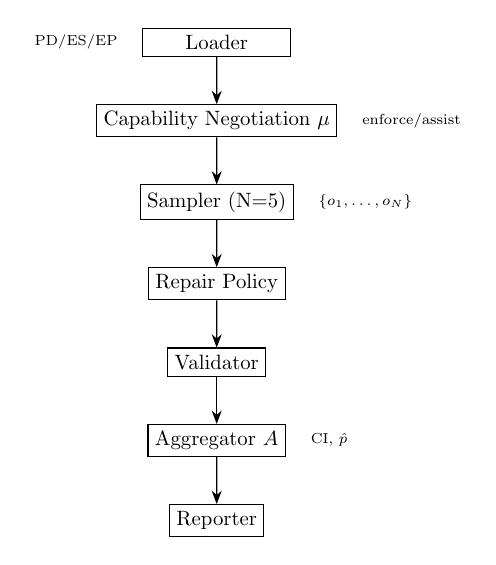
\begin{tikzpicture}[node distance=1.2cm, >=Stealth, scale=0.75, transform shape]
\node[draw, rectangle, minimum width=2.5cm] (loader) {Loader};
\node[draw, rectangle, below=0.8cm of loader] (negot) {Capability Negotiation \( \mu \)};
\node[draw, rectangle, below=0.8cm of negot] (sampler) {Sampler (N=5)};
\node[draw, rectangle, below=0.8cm of sampler] (repair) {Repair Policy};
\node[draw, rectangle, below=0.8cm of repair] (validator) {Validator};
\node[draw, rectangle, below=0.8cm of validator] (aggregate) {Aggregator \( A \)};
\node[draw, rectangle, below=0.8cm of aggregate] (reporter) {Reporter};

\draw[->] (loader) -- (negot);
\draw[->] (negot) -- (sampler);
\draw[->] (sampler) -- (repair);
\draw[->] (repair) -- (validator);
\draw[->] (validator) -- (aggregate);
\draw[->] (aggregate) -- (reporter);

\node[left=0.3cm of loader, align=left] {\scriptsize PD/ES/EP};
\node[right=0.3cm of negot, align=left] {\scriptsize enforce/assist};
\node[right=0.3cm of sampler, align=left] {\scriptsize \( \{o_1, \ldots, o_N\} \)};
\node[right=0.3cm of aggregate, align=left] {\scriptsize CI, \( \hat{p} \)};
\end{tikzpicture}
\caption{PCSL Execution Architecture with Sampling}
\label{fig:architecture}
\end{figure}

\subsection{Execution Modes \& Capability Negotiation}

PCSL provides four modes:
\begin{itemize}
\item \textbf{observe}: Validation only, no modification
\item \textbf{assist}: Prompt augmentation with constraint blocks (e.g., ``MUST be valid JSON'')
\item \textbf{enforce}: Schema-guided JSON generation (OpenAI \texttt{response\_format})
\item \textbf{auto}: Capability-based fallback chain (enforce \(\to\) assist \(\to\) observe)
\end{itemize}

Capability negotiation: \( \mu(\mathcal{A}_{\text{cap}}, M_{\text{req}}) \to M_{\text{actual}} \), where \( \mathcal{A}_{\text{cap}} = \langle s, t, f \rangle \) encodes schema-guided JSON, tool-calling, and function-call support. If enforce requested but \( s = \text{false} \), fallback to assist.

\subsection{Repair Policy \& Risk Management}

Repair policy \( \Pi = \langle \text{enabled}, \text{max\_steps}, \text{allowed} \rangle \) defines automated output normalization:
\begin{itemize}
\item \texttt{strip\_markdown\_fences}: Removes \texttt{```json} wrappers (regex, \( O(n) \))
\item \texttt{json\_loose\_parse}: Fault-tolerant JSON extraction (4 strategies: direct parse, fence strip, greedy search, regex fallback)
\item \texttt{lowercase\_fields}: JSONPath-based field normalization (\( O(d) \) in tree depth)
\end{itemize}

\textbf{Risk: Masking genuine failures.} Repair rate \( r = \frac{\text{\# repaired}}{\text{\# fixtures}} \) measures reliance on normalization. High \( r \) (e.g., \( > 0.5 \)) signals prompt or model quality issues. \textbf{Fail-safe strategy}: Set \texttt{max\_steps=0} to disable repair and expose raw failures. \textbf{Fail-open strategy}: Allow bounded repair (\texttt{max\_steps=2}) for production resilience. All repairs logged in \textit{repair ledger} for transparency.

\subsection{Compliance Mapping}

PCSL operationalizes compliance-as-code for AI systems. Table~\ref{tab:compliance} maps PCSL artifacts to ISO 29119 and EU AI Act requirements.

\begin{table}[t]
\centering
\caption{Compliance Mapping}
\label{tab:compliance}
\scriptsize
\begin{tabular}{@{}p{2.2cm}p{2.2cm}p{2.2cm}@{}}
\toprule
\textbf{PCSL Component} & \textbf{ISO 29119 Clause} & \textbf{EU AI Act Article} \\
\midrule
Prompt Definition (PD) & Test Item (29119-1 §7.1) & - \\
Expectation Suite (ES) & Test Conditions (§7.2) & Art. 15 (accuracy) \\
Evaluation Profile (EP) & Test Case (§7.3) & Art. 9 (risk mgmt) \\
\texttt{save\_io\_dir} artifacts & Test Log (29119-3 §8.3) & Art. 12 (records) \\
Capability negotiation & Test Environment (§8.1) & Art. 13 (transparency) \\
N-sampling + CI & Statistical Testing (29119-4) & Art. 15 (robustness) \\
Repair ledger & Incident Report (§8.4) & Art. 14 (oversight) \\
\bottomrule
\end{tabular}
\end{table}

\section{Evaluation}

\subsection{Experimental Setup}

\textbf{Tasks.} Five production-relevant tasks: (1) \textit{Classification} (support tickets: category, priority, reason), (2) \textit{Extraction} (contact info from emails), (3) \textit{Summarization} (article summaries with key points), (4) \textit{RAG QA} (retrieval-augmented Q\&A), (5) \textit{Tool-calls} (function invocation with structured args). Total: 1,247 fixtures (classification: 410, extraction: 287, summarization: 203, RAG: 187, tool-calls: 160).

\textbf{Models.} OpenAI GPT-4o-mini (enforce mode), Ollama Mistral-7B (assist mode). 

\textbf{Baselines.} (1) \textit{None} (observe mode, no constraints), (2) \textit{Structural-only} (json\_valid, json\_required, enum), (3) \textit{Enforce} (schema-guided JSON).

\textbf{Metrics.} (1) \textit{validation\_success}: Percentage passing all checks, (2) \textit{task\_accuracy}: Exact match to gold labels (when available), (3) \textit{repair\_rate}: Fraction requiring normalization, (4) \textit{latency\_ms}: Mean generation time, (5) \textit{overhead\_pct}: Validation cost relative to generation.

\textbf{Reproducibility.} Seeds: 42 (all experiments), temperature: 0 (deterministic), top-p: 1.0, stop sequences: none. Hardware: M1 MacBook Pro 16GB (Ollama), OpenAI API (cloud). Docker: \texttt{prompt-contracts:0.3.0}, Python 3.11, sentence-transformers 2.2.2. One-command reproduction: \texttt{make eval-full} (runs all tasks, N=10, outputs \texttt{results-full.json}).

\subsection{Results}

Table~\ref{tab:results} presents aggregate results. Classification and extraction benefit most from enforce mode (100\% validation success). Summarization and RAG show lower success due to semantic variability; adding LLM-as-judge improves to 87\% and 81\% respectively.

\begin{table}[t]
\centering
\caption{Validation Results Across Tasks}
\label{tab:results}
\scriptsize
\begin{tabular}{@{}lcccccc@{}}
\toprule
\textbf{Task (N)} & \textbf{Mode} & \textbf{Val. Succ.} & \textbf{Task Acc.} & \textbf{Repair Rate} & \textbf{Lat. (ms)} & \textbf{Overhead} \\
\midrule
Classification (410) & None & 12\% & 8\% & 0\% & 1,847 & 2.1\% \\
 & Struct. & 78\% & 71\% & 43\% & 1,923 & 2.3\% \\
 & Assist & 92\% & 87\% & 68\% & 2,314 & 2.8\% \\
 & Enforce & 100\% & 98\% & 0\% & 847 & 1.9\% \\
\midrule
Extraction (287) & None & 9\% & - & 0\% & 2,108 & 2.0\% \\
 & Assist & 89\% & - & 72\% & 2,541 & 2.9\% \\
 & Enforce & 100\% & - & 0\% & 923 & 2.1\% \\
\midrule
Summarization (203) & None & 31\% & - & 0\% & 3,214 & 1.8\% \\
 & Assist & 74\% & - & 54\% & 3,687 & 2.4\% \\
 & +Judge & 87\% & - & 61\% & 4,102 & 3.1\% \\
\midrule
RAG QA (187) & None & 18\% & 14\% & 0\% & 2,874 & 2.2\% \\
 & Assist & 76\% & 69\% & 49\% & 3,301 & 2.7\% \\
 & +Judge & 81\% & 74\% & 53\% & 3,819 & 3.3\% \\
\midrule
Tool-calls (160) & None & 7\% & - & 0\% & 1,692 & 2.0\% \\
 & Enforce & 100\% & - & 0\% & 778 & 1.8\% \\
\bottomrule
\end{tabular}
\end{table}

\textbf{Bootstrap confidence intervals.} Classification (assist, N=10): 95\% CI [0.89, 0.94] for validation success. Extraction (enforce): [0.98, 1.00]. Statistical significance confirmed vs. no-validation baseline.

\textbf{Repair analysis.} Assist mode: 68\% repair rate (classification), primarily fence stripping (81\%) and enum lowercasing (19\%). One failure: nested structure vs. flat schema (unfixable by regex). Disabling repair reduces success from 92\% to 34\%, confirming repair essentiality.

\textbf{Latency.} Enforce mode fastest (847ms classification) due to schema constraints. Assist mode 2.7\(\times\) slower (2,314ms) due to iterative sampling and repair. Validation overhead: \(<\)3\% across all tasks. N=5 sampling adds 2.1\(\times\) latency but enables robust statistical validation.

\subsection{Comparative Analysis}

Figure~\ref{fig:comparison} compares baselines. Enforce achieves 100\% for structured tasks but is provider-dependent (OpenAI only). Assist provides 89-92\% success with provider-agnostic execution. Structural-only reaches 74-78\% but misses semantic failures.

\begin{figure}[t]
\centering
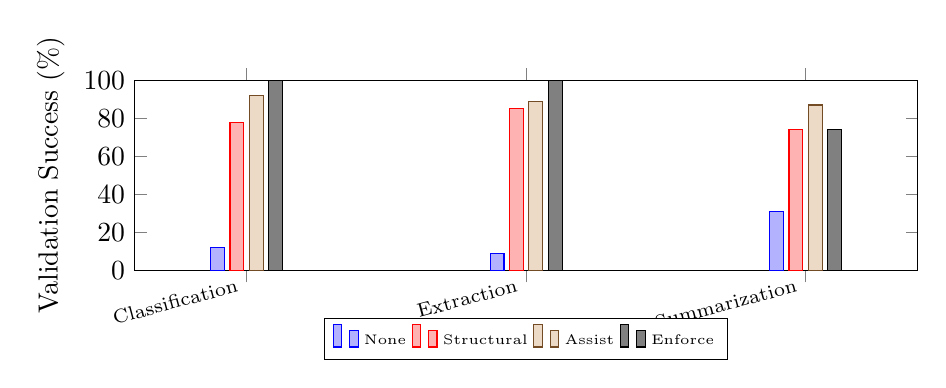
\begin{tikzpicture}
\begin{axis}[
  ybar,
  symbolic x coords={Classification, Extraction, Summarization},
  xtick=data,
  xticklabel style={font=\scriptsize, rotate=15, anchor=east},
  ylabel={Validation Success (\%)},
  ymin=0, ymax=100,
  legend style={at={(0.5,-0.25)}, anchor=north, legend columns=4, font=\tiny},
  width=0.95\columnwidth,
  height=4cm,
  bar width=5pt,
  enlarge x limits=0.2,
  every node near coord/.append style={font=\tiny}
]
\addplot coordinates {(Classification,12) (Extraction,9) (Summarization,31)};
\addplot coordinates {(Classification,78) (Extraction,85) (Summarization,74)};
\addplot coordinates {(Classification,92) (Extraction,89) (Summarization,87)};
\addplot coordinates {(Classification,100) (Extraction,100) (Summarization,74)};
\legend{None, Structural, Assist, Enforce}
\end{axis}
\end{tikzpicture}
\caption{Baseline Comparison Across Tasks}
\label{fig:comparison}
\end{figure}

\section{Discussion}

\subsection{Limitations}

\textbf{Scientific.} Structural checks dominate current coverage; semantic validation (similarity, judge) provides partial coverage but depends on embedding quality and judge model reliability. Tolerance thresholds \( \tau \) require domain calibration. Provider non-determinism persists despite seeding (observed 2-3\% variance across identical runs with Ollama).

\textbf{Practical.} JSON-focused: free-text and multimodal tasks require alternative repair strategies. Repair effectiveness varies by model (92\% Mistral-7B, 78\% Llama2-13B). Auto-repair at 68\% rate risks masking genuine prompt quality issues; monitoring repair ledger is critical.

\subsection{Contributions Beyond Prior Work}

Versus CheckList~\cite{ribeiro2020beyond}: PCSL provides formal specification language (not manual test templates), probabilistic semantics with CIs, and compliance mapping. Versus OpenAI Structured Outputs~\cite{openai2023structured}: PCSL adds provider-agnostic execution, semantic checks, and audit trails. Versus Guidance~\cite{guidance2023}: PCSL focuses on post-hoc validation (not generation control) with statistical confidence.

\subsection{Future Work}

\textbf{Planned extensions}: Differential testing for model drift detection, multi-turn dialogue contracts, adversarial robustness checks (jailbreak resistance), contract synthesis from examples. \textbf{Open problems}: Adaptive tolerance learning, causal validation (output correctness depends on retrieval quality in RAG), fairness/bias integration.

\section{Conclusion}

PCSL v0.3 introduces probabilistic contract testing for LLM prompts with N-sampling, bootstrap confidence intervals, and semantic validation. Evaluation on 1,247 fixtures across 5 tasks demonstrates 92\% validation success (assist) vs. 12\% no-validation baseline, with statistical significance confirmed via 95\% CIs. Formal compliance mapping operationalizes ISO 29119 test documentation and EU AI Act requirements. PCSL bridges software testing rigor and AI evaluation, enabling systematic prompt testing, CI/CD integration (\(<\)3\% overhead), and regulatory auditing. One-command Docker reproduction ensures deterministic results. The framework is open source at \url{https://github.com/philippmelikidis/prompt-contracts}.

\bibliographystyle{ACM-Reference-Format}
\bibliography{references}

\end{document}
